% "Станет проще"

\documentclass[a4paper,12pt]{article} % тип документа

% report, book

% Рисунки
\usepackage{graphicx}
\usepackage{wrapfig}
\usepackage{hyperref}
\usepackage[rgb]{xcolor}



%  Русский язык

\usepackage[T2A]{fontenc}			% кодировка
\usepackage[utf8]{inputenc}			% кодировка исходного текста
\usepackage[english,russian]{babel}	% локализация и переносы


% Математика
\usepackage{amsmath,amsfonts,amssymb,amsthm,mathtools} 


\usepackage{wasysym}

%Заговолок
\author{Сафиуллин Роберт	}
\title{Лабораторная работа 3.4.2\\ Закон Кюри-Вейсса}






\begin{document} % начало документа

\maketitle


\newpage
\section{Цель работы:}
  Изучение температурной зависимости магнитной восприимчивости ферромагнетика выше точки Кюри.\\
\section{В работе используются:}
Катушка самоиндукции с образцом из гадолиния, термостат, частотомер, цифровой вольтметр, LC-автогенератор, термопара медь-константан.

 
\section{Экспериментальная установка:}

 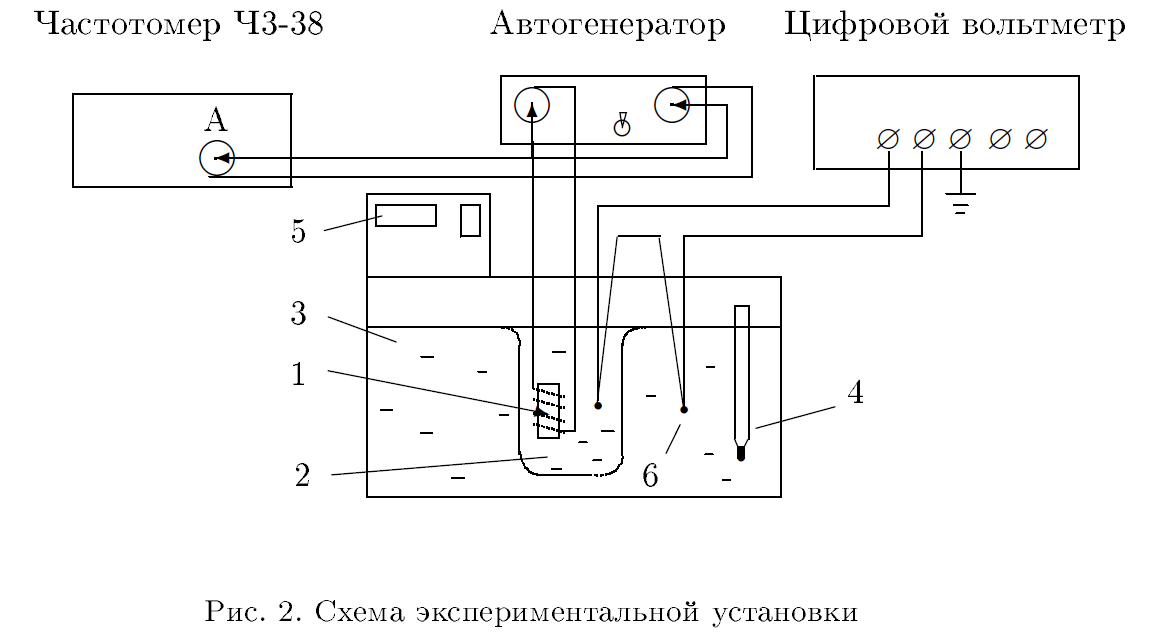
\includegraphics[scale=0.6]{ust}
\section{Ход работы}
1) Подготовили приборы к работе \\
2) Оценили допустимую ЭДС термопары:\\
\begin{equation}
 U=\frac{\Delta T}{k} = \frac{0.5}{24}=0.02 mV
\end{equation}
3) Исследуем зависимость периода колебаний LC-генератора от температуры образца\\
4) Повышая температуру от 14 $C^{o}$ до 40 $C^{o}$ снимем показания вольтметра и частотомера, учтя показания термопары \\($\tau_0$=6.9 мс ). Результаты запишем в таблицу: \\
f(T)=$\frac{1}{(\tau-\tau_0)^{2}}$ \\
\begin{tabular}{|c|c|c|c|c|}
\hline 
$T_{izm}$ $C^{o}$ & T $C^{o}$ & $\tau$, мс & U, mV & f(T)*$10^{-6}$, $c^{-1}$ \\ 
\hline 
16.03 & 15.53 & 7.872 & -0.018 & 0.069 \\ 
\hline 
18.07 & 17.57 & 7.763 & -0.023 & 0.079 \\ 
\hline 
20.01 & 19.51 & 7.63 & -0.035 & 0.094 \\ 
\hline 
22.00 & 21.5 & 7.449 & -0.037 & 0.127 \\ 
\hline 
24.01 & 23.51 & 7.243 & -0.04 & 0.206 \\ 
\hline 
26.01 & 25.51 & 7.126 & -0.036 & 0.315 \\ 
\hline 
28.02 & 27.52 & 7.07 & -0.028 & 0.421 \\ 
\hline 
30.03 & 29.53 & 7.043 & -0.032 & 0.501 \\ 
\hline 
32.04 & 31.54 & 7.02 & -0.029 & 0.598 \\ 
\hline 
34.02 & 33.52 & 7.007 & -0.03 & 0.672 \\ 
\hline 
36.01 & 35.51 & 6.995 & -0.029 & 0.757 \\ 
\hline 
38.01 & 37.51 & 6.985 & -0.03 & 0.847 \\ 
\hline 
40.01 & 39.51 & 6.976 & -0.029 & 0.948 \\ 
\hline 
\end{tabular} 

5) Построим по этим данным график f(T): \\
\begin{flushleft}


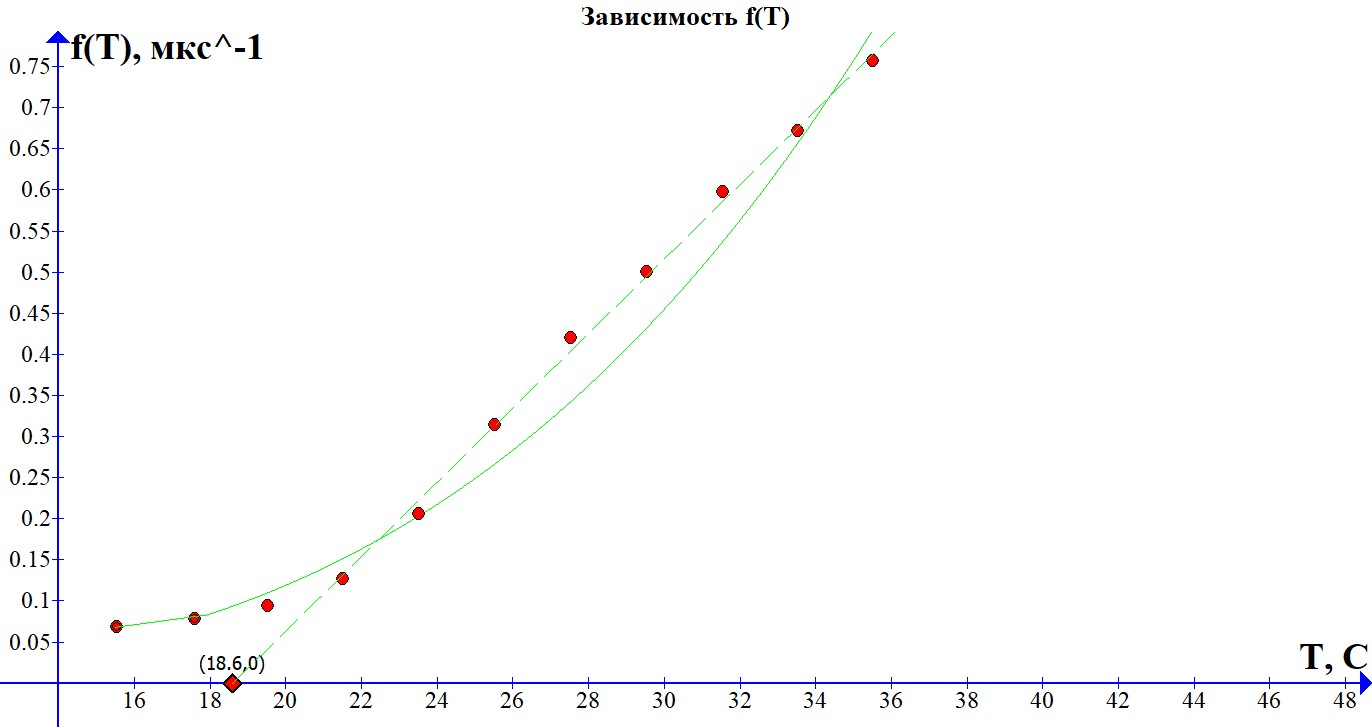
\includegraphics[scale=0.29]{3421}


\end{flushleft}

6) Экстраполируя полученную прямую, получаем точку Кюри: \\
T=18.6 $C^{o}$, при табличном значении: $T_0$=19 $C^{o}$. Полученная температура довольно близка к табличному, но не совпадает полностью, так как данный метод не позволяет получить точное значение точки Кюри.
















































\end{document} % конец документа
